% ---------
% --------
%!TEX TS-program = pdflatex
%!TEX encoding = UTF-8 Unicode
%!TEX spellcheck = English (Aspell)
\documentclass[11pt]{article}
\usepackage{lucy,handout,graphicx}
\usepackage[utf8]{inputenc}		% Allow some non-ASCII Unicode in
\usepackage{tikz}

\def\Cdot{\mathbin{\text{\normalfont \textbullet}}}
\def\Sym#1{\texttt{\color{BrickRed}#1}}
\def\BlueSym#1{\textbf{\texttt{\color{RoyalBlue}#1}}}
\allowdisplaybreaks

\newtheorem{theorem}{Claim}

% =========================================================
%   Define common stuff for solution headers
% =========================================================
\Class{CSCI 332}
\Semester{Fall 2026}

% =========================================================
\begin{document}

% ---------------------------------------------------------



\headers{CSCI 332}{Homework 4 Solutions}{Fall 2026}
\begin{enumerate}

\item Write the recurrence describing the following algorithm's runtime.

\begin{algo}
    Alg(array $A$ of length $n$):\+ \\
        If $n = 1$: \+ \\
            Return $A$ \- \\
        Else: \+ \\
            Return Alg(array formed by taking the values at odd indices of $A$)
\end{algo}

\begin{Solution}
    \begin{equation*}
        T(n) =
        \begin{cases}
        1 & $if $ n = 1 \\
        T(\frac{n}{2}) + n & $if $ n > 1 \\
        \end{cases}
    \end{equation*}
    Note: the $n$ non-recursive work accounts for the runtime to find the odd indices of $A$. We also
    accepted $1$ as the non-recursive work, in case you considered it constant time to process the array.

\end{Solution}

\item Suppose you are given a stack of $n$ pancakes of different sizes. You want to
sort the pancakes so that smaller pancakes are on top of larger pancakes.
The only operation you can perform is a \emph{flip}---insert a spatula
under the top $k$ pancakes, for some integer $k$ between 1 and $n$, and flip them all over.

\begin{figure}[h!]
    \begin{center}
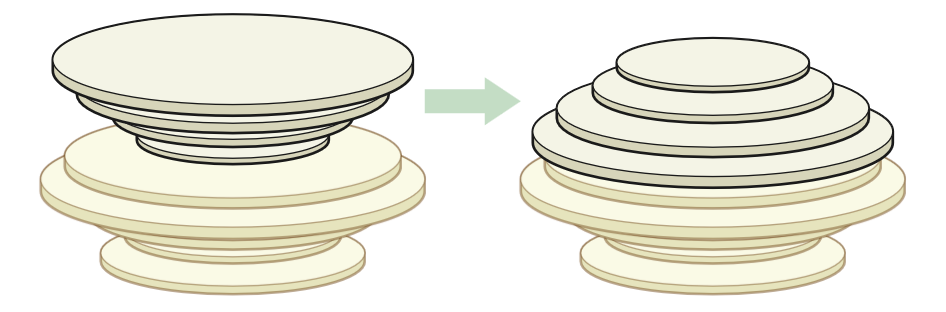
\includegraphics[width=.5\textwidth]{pancakes.png}
    \end{center}
    \caption{Flipping the top four pancakes.}
\end{figure}

\begin{enumerate}
    \item Let $PancakeSort$ be an algorithm that sorts a stack of pancakes. Given a stack of
    $n$ pancakes $S$, describe how you could perform a constant number of flips on $S$
    so that calling $PancakeSort$ on the top $n-1$ pancakes completes the sorting of $S$.
    \begin{Solution}
        We want to get the largest pancake to the bottom of the stack. To do so,
        we can find the largest pancake, insert our spatula just below it, and flip it to the
        top, and then flip the entire stack so that it is on the bottom.
        Now, we can run $PancakeSort$ on the top $n-1$ pancakes to complete the sorting of $S$,
        as required.
    \end{Solution}
    \newpage
    \item Write the full recursive $PancakeSort$ algorithm.

    \begin{Solution}~

        \begin{algo}
            Alg(stack $S$ of $n$ pancakes):\+ \\
                If $n = 1$: \+ \\
                    Return $S$ \- \\
                Else: \+ \\
                    Find the largest pancake in $S$ and flip it to the top of
                    the stack. \\
                    Flip the entire stack so that the largest pancake is on the bottom. \\
                    Return Alg(stack formed by taking the top $n-1$ pancakes of $S$)
        \end{algo}
    \end{Solution}
    \item Write the recurrence for your $PancakeSort$ algorithm's runtime $T(n)$.
    \begin{Solution}
        \begin{equation*}
            T(n) =
            \begin{cases}
            1 & $if $ n = 1 \\
            T(n-1) + n & $if $ n > 1 \\
            \end{cases}
        \end{equation*}
        Note: the $n$ non-recursive work accounts for the runtime to find the
        largest pancake and perform the necessary flips.
    \end{Solution}
\end{enumerate}


\end{enumerate}

\end{document}

